\documentclass[conference]{IEEEtran}
\IEEEoverridecommandlockouts
\usepackage{cite}
\usepackage{amsmath,amssymb,amsfonts}
\usepackage{algorithm}
\usepackage{algpseudocode}
\usepackage{graphicx}
\usepackage{booktabs}
\usepackage{multirow}
\usepackage{textcomp}
\usepackage{xcolor}
\usepackage{tikz}
\usetikzlibrary{arrows.meta,positioning,fit,calc}
\usepackage[hidelinks]{hyperref}

\newcommand{\IND}{\textsc{Ind}}
\newcommand{\CLM}{\textsc{Clm}}
\newcommand{\PRone}{\textsc{PR-1}}
\newcommand{\PRk}{\textsc{PR-k}}
\newcommand{\HUN}{\textsc{Hun}}

\begin{document}

\title{How Much Talk Does a Rescue Team Need? Decomposing the Value of Communication in Decentralized Multi-Agent Disaster Response}

\author{\IEEEauthorblockN{Aahil Sayed \quad Parth Bisen \quad Prachi Pawar \quad Tanvi Patil}
\IEEEauthorblockA{\textit{Department of Computer Engineering, Pimpri Chinchwad College of Engineering (PCCOE)}\\
Pune, India}}

\maketitle

\begin{abstract}
When several autonomous rescue units serve one disaster area, the cheapest way to lose time is for two of them to drive to the same victim. Coordination protocols prevent this, but they differ sharply in communication cost and centralization, and post-disaster networks are lossy. We ask which part of coordination actually buys the gain, and how the answer changes with team size and message loss. We extend RESQ-MAS, an open multi-agent rescue simulator, into a testbed of five allocation protocols of increasing communication cost: independent selection, claim broadcasting, one-round and iterative propose--resolve negotiation, and a centralized Hungarian matcher. Across 28,300 paired simulations on random worlds, one-round negotiation cuts mission completion time by 29.0\% for two agents (1,000 worlds, Holm-corrected Wilcoxon $p<10^{-4}$) and by up to 66\% for eight. Three findings stand out. First, uncoordinated teams saturate: eight independent agents are only 1.7--2.5$\times$ faster than one, against 5.0--6.7$\times$ for negotiating teams, so the empirical price of anarchy grows from 1.3 to 3.1 with team size. Second, the value of negotiation over claim broadcasting is set by contention: 4\% of the total gain at 15 victims per agent, 61\% at 3. Third, iterative negotiation is statistically indistinguishable from the centralized matcher in all 15 team/workload configurations while sending 3--11$\times$ less data, and under broadcast loss every protocol degrades smoothly, retaining roughly a $(1-p)$ fraction of its gain. The testbed and all raw runs are released.
\end{abstract}

\begin{IEEEkeywords}
Multi-agent systems, multi-robot task allocation, disaster response, search and rescue, decentralized coordination, auction algorithms, Hungarian algorithm, price of anarchy, lossy communication, agent-based simulation.
\end{IEEEkeywords}

% ---------------------------------------------------------------------------
\begin{figure}[!t]
\centering
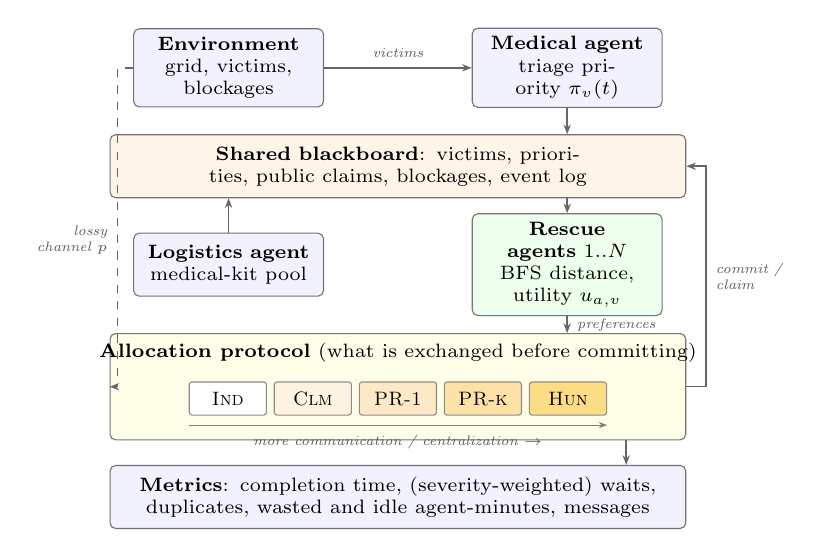
\begin{tikzpicture}[
  font=\scriptsize,
  box/.style={draw=black!55, rounded corners=2pt, fill=#1, align=center, inner sep=3pt, minimum height=0.8cm},
  box/.default=blue!5,
  chip/.style={draw=black!45, rounded corners=1pt, fill=#1, minimum width=0.98cm, minimum height=0.42cm, inner sep=1pt, font=\scriptsize},
  lbl/.style={font=\tiny\itshape, text=black!65},
  arr/.style={-{Stealth[length=3.5pt]}, black!60, line width=0.55pt}]
\node[box, text width=2.2cm] (env) at (0,0) {\textbf{Environment}\\grid, victims, blockages};
\node[box, text width=2.2cm] (med) at (4.3,0) {\textbf{Medical agent}\\triage priority $\pi_v(t)$};
\node[box=orange!9, text width=7.1cm] (bb) at (2.15,-1.25) {\textbf{Shared blackboard}: victims, priorities, public claims, blockages, event log};
\node[box, text width=2.2cm] (log) at (0,-2.5) {\textbf{Logistics agent}\\medical-kit pool};
\node[box=green!7, text width=2.2cm] (ra) at (4.3,-2.5) {\textbf{Rescue agents} $1..N$\\BFS distance, utility $u_{a,v}$};
\node[box=yellow!9, text width=7.1cm, minimum height=1.35cm] (proto) at (2.15,-4.05) {};
\node[anchor=north, font=\scriptsize] at (proto.north) {\textbf{Allocation protocol} (what is exchanged before committing)};
\foreach \name/\shade [count=\i] in {\IND/0,\CLM/10,\PRone/20,\PRk/32,\HUN/45}
  \node[chip=yellow!\shade!orange!\shade] (c\i) at ({-1.09+1.08*\i},-4.2) {\name};
\draw[-{Stealth[length=3pt]}, black!50] ($(c1.south west)+(0,-0.12)$) -- node[below, lbl, pos=0.5]{more communication / centralization $\rightarrow$} ($(c5.south east)+(0,-0.12)$);
\node[box, text width=7.1cm] (met) at (2.15,-5.45) {\textbf{Metrics}: completion time, (severity-weighted) waits, duplicates, wasted and idle agent-minutes, messages};
\draw[arr] (env) -- node[above, lbl]{victims} (med);
\draw[arr] (med) -- (med|-bb.north);
\draw[arr] (bb.south-|ra) -- (ra);
\draw[arr] (log) -- (log|-bb.south);
\draw[arr] (ra) -- node[right, lbl]{preferences} (ra|-proto.north);
\draw[arr] (proto.east) -- ++(0.25,0) |- node[pos=0.25, right, lbl, align=left]{commit /\\claim} (bb.east);
\draw[arr] ($(proto.south)+(2.9,0)$) -- ($(met.north)+(2.9,0)$);
\draw[arr, dashed] (env.west) -- ++(-0.2,0) |- node[pos=0.27, left, lbl, align=right]{lossy\\channel $p$} (proto.west);
\end{tikzpicture}
\caption{RESQ-MAS testbed. The world is generated deterministically from a seed, so every protocol runs on an identical world (paired design). The medical agent publishes priorities to a shared blackboard; rescue agents score reachable victims and hand their preferences to one of five allocation protocols that differ only in what is communicated before an agent commits. Routing, replanning, pickup, and delivery are shared code, so any metric difference is attributable to the protocol alone.}
\label{fig:arch}
\end{figure}

% ---------------------------------------------------------------------------
\section{Introduction}
After an earthquake or flood, emergency operations centers dispatch ambulances, ground robots, and drones to many casualties at once, often over degraded radio links and with little time for central planning~\cite{queralta2020,kitano1999}. A recurring and expensive failure mode in such operations is \emph{duplicated effort}: two units independently decide that the same critical victim is the most urgent, both travel there, and one arrives to find nothing to do while other victims keep waiting. Multi-agent coordination research offers many remedies, from market-based auctions~\cite{smith1980,gerkey2002,dias2006} to consensus protocols~\cite{choi2009} and optimal centralized assignment~\cite{kuhn1955}. What a practitioner designing a dispatch system actually needs to know, however, is more specific: \emph{which part} of coordination produces the benefit, \emph{how much communication} it costs, and \emph{how it behaves} when messages are lost.

This paper answers these questions with a controlled, paired simulation study. Our starting point is RESQ-MAS, an open-source disaster-rescue simulator in which a medical triage agent, a logistics agent, and a team of rescue agents interact through a shared blackboard~\cite{hayesroth1985}. Its original release compared two policies on 20 hand-picked runs. We extend it into a protocol testbed (Fig.~\ref{fig:arch}) with five allocation protocols ordered by communication cost, support for arbitrary team sizes, an explicit lossy-broadcast model, and instrumentation for wasted effort and message volume, and we evaluate it on 28,300 simulations over randomly generated worlds.

\subsection{Contributions}
\begin{itemize}
\item A \textbf{communication ladder} of five task-allocation protocols implemented on one shared agent codebase, so that the \emph{only} difference between conditions is what agents exchange before committing: nothing, public claims, one negotiation round, iterative negotiation, or full utility reports to a centralized optimal matcher.
\item A \textbf{decomposition of the coordination gain} into a claim-broadcasting component and a same-tick negotiation component, showing that the share due to negotiation is governed by the contention ratio between agents and victims (4\% to 61\%).
\item Evidence that \textbf{uncoordinated teams saturate}: adding agents without coordination yields at most 2.5$\times$ speedup at eight agents, and the empirical price of anarchy grows roughly linearly with team size.
\item Evidence that \textbf{decentralized iterative negotiation matches a centralized matcher} in all 15 tested configurations (no significant difference after Holm correction) with 3--11$\times$ lower communication volume, and that all message-based protocols degrade gracefully under broadcast loss.
\item A reproducible, open testbed with fixed seeds, paired statistics, and all raw runs released.
\end{itemize}

% ---------------------------------------------------------------------------
\section{Related Work}
\subsection{Multi-Robot Task Allocation}
Gerkey and Matari\'c~\cite{gerkey2004} classify multi-robot task allocation (MRTA) problems; our setting, in which each agent serves one victim at a time and victims are revealed up front, is the single-task, single-robot, instantaneous-assignment (ST-SR-IA) class, repeated over time as agents become free. ST-SR-IA reduces to the linear assignment problem, solvable optimally by the Hungarian method~\cite{kuhn1955} or distributedly by Bertsekas' auction algorithm~\cite{bertsekas1988}. Market-based approaches descend from the Contract Net protocol~\cite{smith1980}; Gerkey and Matari\'c's MURDOCH~\cite{gerkey2002}, the survey by Dias \emph{et al.}~\cite{dias2006}, and sequential single-item auctions~\cite{lagoudakis2005,koenig2010} show that greedy auctions achieve near-optimal team performance at low communication cost. Behaviour-based architectures such as ALLIANCE~\cite{parker1998} coordinate implicitly through broadcast of current activity, which corresponds to the claim-broadcasting rung of our ladder.

\subsection{Coordination for Disaster Rescue}
RoboCup Rescue~\cite{kitano1999} established urban search and rescue as a benchmark domain for multi-agent research, and Ramchurn \emph{et al.}~\cite{ramchurn2010} demonstrated decentralized coordination of ambulance and fire-brigade agents in it using max-sum message passing. Queralta \emph{et al.}~\cite{queralta2020} survey multi-robot search-and-rescue systems and identify coordination under unreliable communication as an open operational concern.

\subsection{Coordination under Limited Communication}
Choi \emph{et al.}~\cite{choi2009} proved that the consensus-based auction algorithm converges to conflict-free assignments under network-topology changes. Otte \emph{et al.}~\cite{otte2020} studied several auction variants under message loss and found that auction performance degrades gracefully with increasing loss. The price-of-anarchy concept of Koutsoupias and Papadimitriou~\cite{koutsoupias1999}, the ratio between the cost of uncoordinated equilibria and the social optimum, gives a natural lens for quantifying what coordination is worth.

\subsection{Research Gap}
Existing studies typically propose one protocol and compare it against a baseline, so the \emph{marginal} value of each additional kind of communication is rarely isolated. The scaling of that value with team size, the role of contention, and the cost of centralization are usually reported, if at all, for a single configuration. Table~\ref{tab:position} positions this paper.

\begin{table}[!t]
\caption{Positioning Relative to Reviewed Work}
\label{tab:position}
\centering
\footnotesize
\setlength{\tabcolsep}{3pt}
\begin{tabular}{@{}p{1.55cm}p{2.25cm}p{3.95cm}@{}}
\toprule
\textbf{Study} & \textbf{Focus} & \textbf{Gap addressed here} \\
\midrule
Gerkey \cite{gerkey2004} & MRTA taxonomy & Formal analysis; no empirical ladder of protocols \\
Koenig \cite{koenig2010}, Lagoudakis \cite{lagoudakis2005} & Sequential auctions & Routing costs; no rescue priorities or message loss \\
Choi \cite{choi2009} & Consensus auctions & Convergence proofs; no decomposition of the gain \\
Ramchurn \cite{ramchurn2010} & RoboCup Rescue, max-sum & One protocol; no scaling or centralization comparison \\
Otte \cite{otte2020} & Auctions under loss & No claim-only or independent baselines on same code \\
\textbf{This paper} & Five-rung ladder, 28.3k paired runs & Decomposition, scaling law, optimality gap, loss robustness \\
\bottomrule
\end{tabular}
\end{table}

% ---------------------------------------------------------------------------
\section{System Model}
\subsection{Environment}
The world is a $W\times W$ 4-connected grid ($W=15$ or $20$) in which about 10\% of cells are buildings, one cell is a hospital, and two corner cells are depots from which rescue agents start. $M$ victims are placed on random road cells with severities drawn from \{critical, high, moderate, low\} with probabilities $\{0.2,0.3,0.3,0.2\}$. A fraction $b$ of free road cells is scheduled to become blocked at a random time in the first 120 simulated minutes and to reopen 10--75 minutes later; blockages are published to all agents immediately and trigger BFS replanning. One tick represents one simulated minute. A victim counts as rescued when delivered to the hospital; each rescue consumes one medical kit, allocated by the logistics agent, which refuses a second kit for a victim that already holds one. An agent whose target has been rescued by someone else, or whose kit request stays denied for 40 ticks, abandons that target.

\subsection{Priorities and Utility}
The medical agent republishes each waiting victim's priority as
\begin{equation}
\pi_v(t) = s_v + \lambda\, w_v(t),
\label{eq:priority}
\end{equation}
where $s_v\in\{4,3,2,1\}$ is the severity score, $w_v(t)$ the waiting time so far, and $\lambda=0.1$, so severity dominates but long-waiting victims eventually rise. An idle agent $a$ scores every reachable candidate victim $v$ by
\begin{equation}
u_{a,v}(t) = \pi_v(t) - \beta\, d_a(v),
\label{eq:utility}
\end{equation}
with $d_a(v)$ the BFS shortest-path length on the currently known grid and $\beta=0.1$. All protocols use the same utility; they differ only in how preferences are turned into commitments.

\subsection{The Communication Ladder}
\textbf{\IND{} (independent).} Each idle agent commits to its own $\arg\max_v u_{a,v}$ over all unrescued victims. Nothing is communicated, so agents may converge on the same victim or chase a victim already being carried.

\textbf{\CLM{} (claim broadcasting).} After committing, an agent broadcasts a claim; other agents exclude claimed victims from their candidate sets. Choices made in the same tick are not negotiated, so simultaneous duplicates remain possible. This mirrors activity broadcasting in behaviour-based architectures~\cite{parker1998}.

\textbf{\PRone{} (one-round propose--resolve).} Idle agents first broadcast a proposal $(v, u_{a,v})$. Proposals for the same victim are resolved deterministically: highest utility wins, ties go to shorter distance, then agent identifier. Winners commit and broadcast claims; losers stay idle for the rest of the tick and propose again at the next tick. The resolution rule is a pure function of public messages, so every agent can compute it locally; no privileged coordinator is needed. This is the original RESQ-MAS coordination mechanism.

\textbf{\PRk{} (iterative propose--resolve).} As \PRone{}, but losers immediately re-propose their best victim not yet won in the current tick, repeating until every idle agent holds a target or no candidate remains (Algorithm~\ref{alg:prk}). This is a sequential single-item auction~\cite{koenig2010} executed within one tick.

\textbf{\HUN{} (centralized reference).} Each idle agent reports its full utility row; a coordinator solves $\max \sum_{a,v} u_{a,v}x_{a,v}$ over one-to-one assignments with the Hungarian method~\cite{kuhn1955} (SciPy~\cite{virtanen2020}) and returns the matching. \HUN{} is optimal \emph{per decision epoch}, not over the whole mission, because it re-solves only for currently idle agents and never pre-empts commitments.

\begin{algorithm}[!t]
\caption{\PRk{}: one tick of iterative propose--resolve}
\label{alg:prk}
\small
\begin{algorithmic}[1]
\State $\mathcal{A} \gets$ idle agents; $\mathcal{T} \gets$ victims won this tick
\State each $a\in\mathcal{A}$ proposes $v_a=\arg\max_{v\notin \text{claims}\cup\mathcal{T}} u_{a,v}$
\While{$\mathcal{A}\neq\emptyset$ and some proposal exists}
  \For{each victim $v$ with proposals}
    \State winner $\gets \arg\max (u_{a,v}, -d_a(v), -\text{id}_a)$
    \State winner commits, broadcasts claim; $\mathcal{T}\gets\mathcal{T}\cup\{v\}$
  \EndFor
  \State $\mathcal{A}\gets$ losers; each re-proposes over victims $\notin\mathcal{T}$
\EndWhile
\end{algorithmic}
\end{algorithm}

\subsection{Lossy Broadcast Model}
Every broadcast (proposal or claim) is independently lost with probability $p$ for all receivers, a broadcast-erasure channel. A sender whose proposal is lost hears no objection and commits unilaterally; a lost claim leaves the victim visible as a candidate to others until its delivery to the hospital, which we assume is always observed. Loss draws use a random stream separate from world generation, so lossy and loss-free runs share the same world. At $p=1$ every message-based protocol reduces exactly to \IND{}.

\subsection{Metrics}
Per run we record the completion time $T$ (minute the last victim is delivered), the mean waiting time of rescued victims, a severity-weighted waiting time $\bar w_s=\sum_v s_v w_v / \sum_v s_v$, the mean wait of critical victims, duplicate commitments (distinct victims to which two agents were simultaneously committed), wasted agent-minutes (time spent committed to targets later abandoned), idle agent-minutes while victims remained, and communication as broadcast count and payload (scalar values transmitted). From these we derive the speedup $S(N)=T(1)/T(N)$, the empirical price of anarchy $\mathrm{PoA}=T_{\IND}/T_{\HUN}$, the optimality gap of protocol $X$, $(T_X-T_{\HUN})/T_{\HUN}$, and the \emph{negotiation share} of the coordination gain,
\begin{equation}
\eta = \frac{T_{\CLM} - T_{\PRone}}{T_{\IND} - T_{\PRone}},
\label{eq:eta}
\end{equation}
the fraction of the total \IND{}$\rightarrow$\PRone{} improvement that claim broadcasting alone does not deliver.

% ---------------------------------------------------------------------------
\section{Experimental Design}
All worlds are generated from seeds starting at 1000, disjoint from the curated demonstration seeds of the original release. Each world is run once under every protocol, so all comparisons are paired. Random building placement occasionally walls a victim or the hospital off from both depots; no protocol can rescue such a victim, so these worlds (19 of 1,019 at $W=15$; 7--8 of 157--158 at $W=20$) are excluded deterministically before any run and replaced by the next valid seed. Every retained run rescued every victim.

\textbf{E1 -- Generalization:} $N=2$, $M=6$, $W=15$, 1,000 worlds, $b\in\{0,0.1\}$, all five protocols (10,000 runs). This is the original RESQ-MAS setting on random rather than curated worlds.
\textbf{E2 -- Scaling:} $N\in\{1,2,3,4,6,8\}$, $M\in\{10,20,30\}$, $W=20$, 150 worlds per cell (11,700 runs).
\textbf{E3 -- Message loss:} $N=4$, $M=20$, $p\in\{0,0.05,0.1,0.2,0.3,0.5,0.7,1\}$ for \CLM{}, \PRone{}, \PRk{} (3,600 runs).
\textbf{E4 -- Blockages:} $N=4$, $M=20$, $b\in\{0,0.1,0.2,0.3\}$, all protocols (3,000 runs).

Paired differences are tested with the two-sided Wilcoxon signed-rank test~\cite{wilcoxon1945}, with Holm's step-down correction~\cite{holm1979} applied within each experiment family (36 tests in E1, 45 in E2). Effect sizes are matched-pairs rank-biserial correlations $r_{rb}$~\cite{kerby2014}, and 95\% confidence intervals for mean paired differences use 2,000 bootstrap resamples~\cite{efron1979}. The complete study (28,300 runs) takes about 3.5 minutes on four CPU cores.

% ---------------------------------------------------------------------------
\section{Results}
\subsection{E1: The Original Two-Agent Setting on Random Worlds}
Table~\ref{tab:e1} and Fig.~\ref{fig:e1} summarize E1. On 1,000 random worlds, \PRone{} reduces completion time from 99.3 to 70.5 minutes (29.0\%), mean waiting time by 25.9\%, and severity-weighted waiting time by 23.0\%, and it eliminates duplicate commitments (4.07 per run to 0) and wasted effort (69.9 agent-minutes to 0). The original release reported a 20.9\% completion-time gain on 20 curated runs; the curated benchmark therefore \emph{understated} the effect rather than inflating it. Critical victims, the ones triage protects first under every protocol, still wait 10\% less under negotiation (25.2 to 22.7 min), because agents are no longer tied up on duplicates when a critical victim becomes the best candidate.

\begin{table}[!t]
\caption{E1: Two Agents, Six Victims, 1,000 Random Worlds (Means)}
\label{tab:e1}
\centering
\footnotesize
\setlength{\tabcolsep}{2.6pt}
\begin{tabular}{@{}llrrrrrrr@{}}
\toprule
$b$ & Prot. & $T$ & Wait & $\bar w_s$ & Crit. & Dup. & Waste & Msgs \\
\midrule
0\% & IND & 99.3 & 54.4 & 45.8 & 25.2 & 4.07 & 69.9 & 0.0 \\
0\% & CLM & 88.1 & 50.5 & 43.3 & 25.2 & 2.08 & 43.2 & 8.1 \\
0\% & PR-1 & 70.5 & 40.3 & 35.2 & 22.7 & 0.00 & 0.0 & 20.4 \\
0\% & PR-k & 70.1 & 40.0 & 34.9 & 22.6 & 0.00 & 0.0 & 21.2 \\
0\% & HUN & 69.9 & 39.9 & 34.9 & 22.7 & 0.00 & 0.0 & 57.2 \\
0\% & CBBA & 70.1 & 40.0 & 35.0 & 22.6 & 0.00 & 0.0 & 158.4 \\
\bottomrule

\end{tabular}\\[2pt]
\parbox{\columnwidth}{\scriptsize All times in simulated minutes. $\bar w_s$: severity-weighted wait; Crit.: mean wait of critical victims; Dup.: duplicate commitments per run; Waste: agent-minutes on abandoned targets; Msgs: coordination broadcasts per run.}
\end{table}

\begin{figure}[!t]
\centering
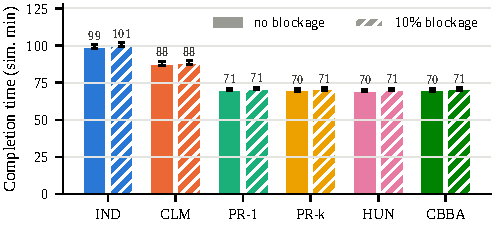
\includegraphics[width=\columnwidth]{figures/fig_e1.pdf}
\caption{E1 completion time per protocol with 95\% confidence intervals (1,000 paired worlds). Solid bars: no blockage; hatched bars: 10\% of road cells blocked mid-run. The ladder improves monotonically, with nearly all of the gain realized by \PRone{}.}
\label{fig:e1}
\end{figure}

Table~\ref{tab:e1tests} decomposes the gain. Claim broadcasting alone recovers 11.2 minutes; one-round negotiation adds a further 17.6. In this high-contention setting (three victims per agent), negotiation contributes 61\% of the total. Beyond \PRone{}, returns vanish: \PRk{} adds 0.4 minutes and \HUN{} a further 0.2. These last differences are statistically detectable with 1,000 pairs, but 91\% of worlds are exact ties between \PRk{} and \HUN{} and the effect size is small ($r_{rb}=0.31$). Adding 10\% blockages changes no conclusion.

\begin{table}[!t]
\caption{E1 Paired Comparisons of Completion Time ($b=0$)}
\label{tab:e1tests}
\centering
\footnotesize
\setlength{\tabcolsep}{2.2pt}
\begin{tabular}{@{}lcrcrcr@{}}
\toprule
Step & $\Delta T$ [95\% CI] & \% & W/T/L & $r_{rb}$ & $p_{\text{Holm}}$ & $\%\bar w_s$ \\
\midrule
IND$\rightarrow$CLM & 11.2 [10.3, 12.1] & 11.3 & 581/385/34 & 0.96 & $<\!10^{-4}$ & 5.3 \\
CLM$\rightarrow$PR-1 & 17.6 [16.5, 18.7] & 20.0 & 741/227/32 & 0.99 & $<\!10^{-4}$ & 18.7 \\
IND$\rightarrow$PR-1 & 28.8 [27.8, 29.9] & 29.0 & 972/4/24 & 1.00 & $<\!10^{-4}$ & 23.0 \\
PR-1$\rightarrow$PR-k & 0.4 [0.4, 0.5] & 0.6 & 436/561/3 & 0.97 & $<\!10^{-4}$ & 0.8 \\
PR-1$\rightarrow$HUN & 0.6 [0.4, 0.7] & 0.8 & 452/518/30 & 0.79 & $<\!10^{-4}$ & 1.1 \\
PR-k$\rightarrow$HUN & 0.2 [0.0, 0.3] & 0.2 & 63/910/27 & 0.31 & 0.019 & 0.3 \\
\bottomrule

\end{tabular}\\[2pt]
\parbox{\columnwidth}{\scriptsize $\Delta T$: mean paired reduction (min). W/T/L: worlds where the second protocol is faster / tied / slower. $\%\bar w_s$: reduction in severity-weighted wait.}
\end{table}

\subsection{E2: Uncoordinated Teams Saturate}
Fig.~\ref{fig:scaling} and Table~\ref{tab:scaling} show the central result. A single agent needs 293, 580, and 870 minutes for 10, 20, and 30 victims. With negotiation, completion time tracks the ideal $T_1/N$ curve closely: eight agents are 5.0--6.7$\times$ faster than one (63--84\% parallel efficiency). Without coordination, eight agents are only 1.7--2.5$\times$ faster, and doubling the team from four to eight buys 3--12\%. The mechanism is visible in Fig.~\ref{fig:waste}(a): independent agents herd onto the same high-priority victims, and wasted effort grows from 241 agent-minutes at $N=2$ to 1,662 at $N=8$ ($M=20$). Consequently the empirical price of anarchy rises almost linearly with team size, from 1.26--1.34 at $N=2$ to 2.80--3.06 at $N=8$, and \PRone{} beats \IND{} on 2,249 of the 2,250 paired worlds with $N\geq 2$, the remaining one being a tie (Holm-corrected $p<10^{-20}$ in every cell). For a dispatcher, the practical reading is blunt: buying more vehicles without a coordination layer delivers a fraction of the capacity paid for.

\begin{figure*}[!t]
\centering
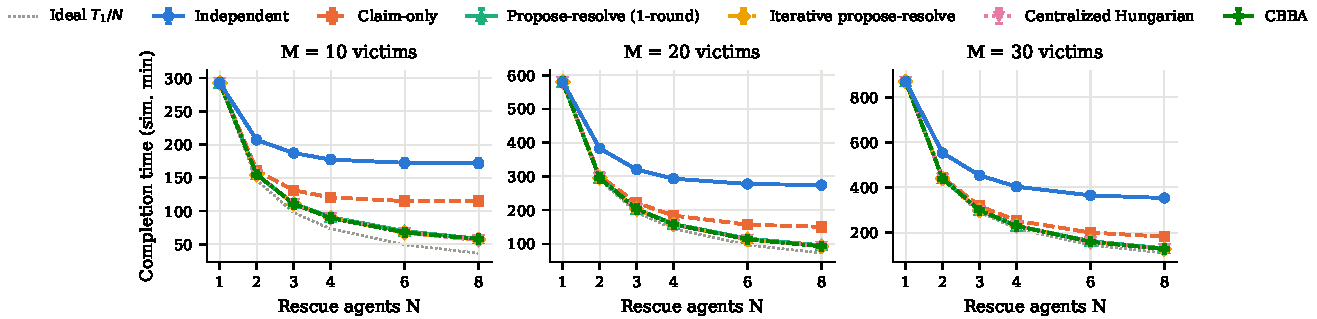
\includegraphics[width=\textwidth]{figures/fig_scaling.pdf}
\caption{E2: completion time versus team size $N$ for three workloads (150 paired worlds per point, 95\% CIs). The dotted grey curve is ideal linear speedup from the single-agent time. Independent agents (blue) flatten after $N\approx 4$; claim broadcasting (orange) recovers part of the gap; the three negotiating protocols overlap and stay close to the ideal curve.}
\label{fig:scaling}
\end{figure*}

\begin{table*}[!t]
\caption{E2: Scaling, Optimality Gap, Negotiation Share, and Communication Volume}
\label{tab:scaling}
\centering
\footnotesize
\setlength{\tabcolsep}{4.2pt}
\begin{tabular}{@{}rrrrrrrrrrrrr@{}}
\toprule
& & \multicolumn{4}{c}{Completion time $T$ (min)} & & \multicolumn{2}{c}{Gap to \HUN{} (\%)} & & \multicolumn{2}{c}{Speedup $S(N)$} & Payload \\
\cmidrule(lr){3-6}\cmidrule(lr){8-9}\cmidrule(lr){11-12}
$M$ & $N$ & \IND{} & \CLM{} & \PRone{} & \HUN{} & PoA & \PRone{} & \PRk{} & $\eta$ (\%) & \IND{} & \PRone{} & \PRone{}/\HUN{} \\
\midrule
10 & 2 & 207 & 161 & 155 & 155 & 1.34 & -0.0 & -0.2 & 11 & 1.41 & 1.89 & 31/132 \\
10 & 4 & 177 & 120 & 91 & 90 & 1.98 & +1.2$^{*}$ & -0.0 & 34 & 1.65 & 3.23 & 41/145 \\
10 & 8 & 172 & 115 & 58 & 56 & 3.06 & +3.7$^{*}$ & +1.2 & 50 & 1.71 & 5.03 & 68/193 \\
\midrule
20 & 2 & 383 & 300 & 295 & 296 & 1.30 & -0.1 & -0.1 & 6 & 1.51 & 1.96 & 61/462 \\
20 & 4 & 293 & 184 & 159 & 158 & 1.86 & +0.7$^{*}$ & -0.0 & 19 & 1.98 & 3.65 & 72/475 \\
20 & 8 & 274 & 150 & 95 & 93 & 2.96 & +2.9$^{*}$ & +0.1 & 31 & 2.11 & 6.07 & 118/532 \\
\midrule
30 & 2 & 553 & 443 & 439 & 440 & 1.26 & -0.1 & -0.1 & 4 & 1.57 & 1.98 & 91/993 \\
30 & 4 & 403 & 253 & 230 & 229 & 1.76 & +0.6$^{*}$ & +0.1 & 13 & 2.16 & 3.78 & 103/1006 \\
30 & 8 & 353 & 182 & 130 & 126 & 2.80 & +2.5$^{*}$ & +0.0 & 23 & 2.46 & 6.71 & 152/1065 \\
\bottomrule

\end{tabular}\\[2pt]
\parbox{\textwidth}{\scriptsize PoA $=T_{\IND}/T_{\HUN}$. Gap: $(T_X-T_{\HUN})/T_{\HUN}$; $^{*}$ marks Holm-corrected Wilcoxon $p<0.05$ (45 tests); negative values mean the protocol beat the per-epoch optimum. $\eta$: negotiation share, Eq.~(\ref{eq:eta}). Payload: scalars transmitted per run. 150 paired worlds per row.}
\end{table*}

\subsection{E2: What Negotiation Adds, and When}
The negotiation share $\eta$ in Table~\ref{tab:scaling} is not a constant. It rises with the ratio of agents to victims: 4--11\% at $N=2$, 13--34\% at $N=4$, and 23--50\% at $N=8$, reaching 61\% in the E1 setting ($M/N=3$). When victims vastly outnumber agents, agents rarely become idle in the same tick with the same favourite, so public claims prevent almost all duplication and \CLM{} is nearly as good as \PRone{}. As contention rises, simultaneous choices collide, claims arrive too late, and the proposal round becomes the decisive ingredient. The design rule is therefore conditional: claim broadcasting is sufficient for sparse, large-area operations, while dense incidents with many units need explicit negotiation.

\subsection{E2: Decentralized Negotiation versus Centralized Optimization}
\PRk{} is statistically indistinguishable from the centralized Hungarian matcher in all 15 $(N,M)$ cells after correction, with mean gaps between $-0.2\%$ and $+1.2\%$. The simpler \PRone{} is within 3.7\% everywhere, but its gap grows with $N$ and is significant in every cell with $N\geq 4$ (and in one of the three $N=3$ cells): each conflict loser idles for one tick, and with more agents there are more losers per tick. The iterative retry of \PRk{} removes exactly this cost. The two negotiation protocols also move far less data than \HUN{}, whose agents must report a utility for every candidate victim: at $M=30$, \PRone{} transmits 91--152 scalars per mission against roughly 1,000 for \HUN{}. Because \HUN{} optimizes only the current epoch, the decentralized protocols occasionally beat it (negative gaps at $N=2$).

Fig.~\ref{fig:waste}(b) shows a side effect worth noting. Coordinated teams accumulate \emph{more} idle agent-minutes than independent ones (230 vs.\ 92 at $N=8$, $M=20$), because once every remaining victim is claimed, the surplus agents correctly wait instead of duplicating. That idle time is uncommitted capacity a dispatcher can redeploy, for example to reconnaissance or to a second incident, whereas the independent team's wasted minutes cannot be recovered.

\begin{figure}[!t]
\centering
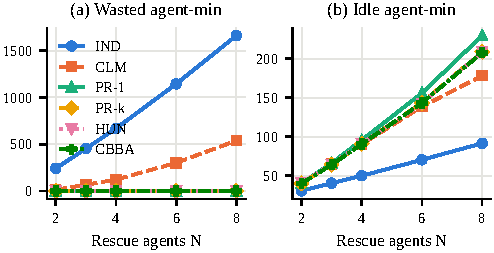
\includegraphics[width=\columnwidth]{figures/fig_waste.pdf}
\caption{E2 ($M=20$): (a) agent-minutes spent on targets later abandoned; (b) agent-minutes idle while victims remained. Negotiation converts wasted travel into idle, redeployable capacity.}
\label{fig:waste}
\end{figure}

\subsection{E3: Robustness to Message Loss}
Fig.~\ref{fig:loss} shows that no protocol collapses under broadcast loss. Completion time rises smoothly from the loss-free value toward the \IND{} level, which all protocols reach exactly at $p=1$, as the model requires. Negotiation retains roughly a $(1-p)$ fraction of its gain over \IND{}: 92\% at $p=0.1$, 73\% at $p=0.3$, and 53\% at $p=0.5$ for \PRone{}. With 10\% of messages lost, \PRone{} is still 42\% faster than independent agents. The margin of negotiation over claim-only shrinks with loss (25.2 minutes at $p=0$, 14.7 at $p=0.5$), because a lost proposal becomes a unilateral commitment. \PRk{} gains relative to \PRone{} as loss grows (8.2 minutes at $p=0.7$), since its within-tick retries give a losing agent another chance to be heard. Duplicate commitments grow almost linearly in $p$ (Fig.~\ref{fig:loss}b), so the duplicate rate is a usable online indicator of link quality.

\begin{figure}[!t]
\centering
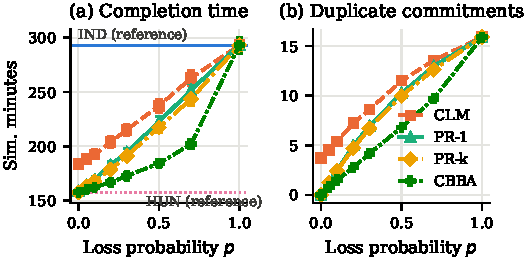
\includegraphics[width=\columnwidth]{figures/fig_loss.pdf}
\caption{E3 ($N=4$, $M=20$, 150 paired worlds per point): (a) completion time and (b) duplicate commitments versus broadcast-loss probability. Horizontal lines give the loss-free \IND{} and \HUN{} references. All protocols converge to \IND{} at $p=1$.}
\label{fig:loss}
\end{figure}

\subsection{E4: Robustness to Road Blockages}
Table~\ref{tab:block} shows that dynamic blockages of up to 30\% of road cells lengthen missions by at most 3.2\% under any protocol and leave the \IND{}$\rightarrow$\PRone{} gain essentially constant at 45--46\%. Blockages affect routing, which every protocol handles with the same BFS replanning, but not the allocation question that separates them.

\begin{table}[!t]
\caption{E4: Completion Time (min) under Road Blockages ($N=4$, $M=20$)}
\label{tab:block}
\centering
\footnotesize
\setlength{\tabcolsep}{3.5pt}
\begin{tabular}{@{}lrrrrrr@{}}
\toprule
$b$ & \IND{} & \CLM{} & \PRone{} & \PRk{} & \HUN{} & Gain (\%) \\
\midrule
0\% & 293.1 & 183.9 & 158.7 & 157.6 & 157.6 & 45.9 \\
10\% & 294.9 & 184.7 & 160.1 & 158.9 & 158.9 & 45.7 \\
20\% & 296.2 & 187.0 & 161.9 & 160.9 & 160.7 & 45.3 \\
30\% & 299.5 & 187.5 & 163.8 & 162.6 & 162.5 & 45.3 \\
\bottomrule

\end{tabular}\\[2pt]
\parbox{\columnwidth}{\scriptsize Gain: \IND{}$\rightarrow$\PRone{} completion-time reduction. 150 paired worlds per row.}
\end{table}

% ---------------------------------------------------------------------------
\section{Discussion}
\subsection{Implications for Dispatch System Design}
Three practical rules follow. \emph{First, coordinate before you scale}: without a coordination layer the marginal value of each added unit falls quickly, so fleet expansion and coordination infrastructure should be planned together. \emph{Second, match the protocol to contention}: when units are few relative to casualties, lightweight claim broadcasting (a status message per dispatch) captures most of the benefit; in dense incidents, add a proposal round. \emph{Third, centralization is not required for near-optimal allocation}: iterative propose--resolve matches a central optimizer with a fraction of the traffic and without a single point of failure, which matters when the operations center itself may be unreachable. These rules apply to ambulance and drone dispatch, warehouse and delivery robot fleets, and any setting where independent agents choose from a shared pool of tasks.

\subsection{Comparison with Existing Work}
Our near-equivalence between iterative negotiation and optimal assignment is consistent with the near-optimality of sequential single-item auctions reported for multi-robot routing~\cite{lagoudakis2005,koenig2010}, and our graceful-degradation result under message loss agrees qualitatively with Otte \emph{et al.}~\cite{otte2020}. What these studies do not provide, and this one does, is the decomposition of the gain on a single codebase, which shows that the value of explicit negotiation is conditional on contention rather than universal.

\subsection{Limitations}
\begin{itemize}
\item The world is a synthetic grid with uniform travel cost, one hospital, one kit per victim, and all victims known at $t=0$. Victim discovery, heterogeneous vehicles, and capacities above one are not modelled.
\item The duplicated-effort penalty depends on simulator rules, in particular the 40-tick kit timeout and the ``already allocated'' kit denial. Different rules would change the absolute size of the \IND{} penalty, although not the fact that duplicates waste effort.
\item \HUN{} is a per-epoch optimum, not a full-horizon optimum; the optimality gaps are relative to that reference.
\item The loss model is independent broadcast erasure. Correlated outages, partitions, and delay are not modelled.
\item Times are simulated minutes produced by the model, not field measurements, and priority weights ($\lambda$, $\beta$) were fixed rather than tuned.
\end{itemize}

\subsection{Future Work}
\begin{itemize}
\item Add staggered victim discovery by a sensing agent, which couples information latency with allocation.
\item Evaluate consensus-based bundle auctions~\cite{choi2009} and max-sum~\cite{ramchurn2010} on the same ladder, including multi-victim capacity.
\item Replace independent loss with partition and delay models derived from post-disaster network measurements.
\item Use the duplicate rate observed online to switch adaptively between claim-only and negotiation modes.
\end{itemize}

% ---------------------------------------------------------------------------
\section{Conclusion}
We asked how much communication a rescue team needs, and answered it with a five-rung communication ladder evaluated on 28,300 paired simulations. Coordination is worth 29\% of mission time for two agents and up to 66\% for eight; without it, teams saturate at 1.7--2.5$\times$ single-agent speed regardless of size. The value splits between broadcasting claims and negotiating simultaneous choices in a ratio set by contention, and a fully decentralized iterative negotiation matches a centralized optimal matcher while sending 3--11$\times$ less data and degrading gracefully as messages are lost. For practitioners the message is simple: the first few bytes of coordination are worth more than the next few vehicles.

\section*{Reproducibility}
Code, fixed seeds, all raw per-run CSV files, and the scripts that generate every table and figure are in the RESQ-MAS repository (\texttt{experiments/study.py}, \texttt{experiments/paper\_figures.py}). The 73-test suite covers every protocol, the loss model, and the optimal matcher.

\section*{Responsible and Ethical Use of AI}
The authors directed the research question, the experimental design, and the interpretation of results. An AI assistant (Claude, Anthropic) was used as an implementation and drafting aid under author direction, and its output was reviewed by the authors. Every number in this paper was produced by code executed against the described simulator; none was estimated or written in by hand. Cited references were checked against their original sources. The authors accept full responsibility for the correctness and integrity of this work.

\begin{thebibliography}{99}
\bibitem{queralta2020} J. Peña Queralta, J. Taipalmaa, B. Can Pullinen, V. K. Sarker, T. Nguyen Gia, H. Tenhunen, M. Gabbouj, J. Raitoharju, and T. Westerlund, ``Collaborative multi-robot search and rescue: Planning, coordination, perception, and active vision,'' \emph{IEEE Access}, vol. 8, pp. 191617--191643, 2020.
\bibitem{kitano1999} H. Kitano, S. Tadokoro, I. Noda, H. Matsubara, T. Takahashi, A. Shinjou, and S. Shimada, ``RoboCup Rescue: Search and rescue in large-scale disasters as a domain for autonomous agents research,'' in \emph{Proc. IEEE Int. Conf. Systems, Man, and Cybernetics}, vol. 6, 1999, pp. 739--743.
\bibitem{smith1980} R. G. Smith, ``The contract net protocol: High-level communication and control in a distributed problem solver,'' \emph{IEEE Trans. Comput.}, vol. C-29, no. 12, pp. 1104--1113, 1980.
\bibitem{gerkey2002} B. P. Gerkey and M. J. Matari\'c, ``Sold!: Auction methods for multirobot coordination,'' \emph{IEEE Trans. Robot. Autom.}, vol. 18, no. 5, pp. 758--768, 2002.
\bibitem{dias2006} M. B. Dias, R. Zlot, N. Kalra, and A. Stentz, ``Market-based multirobot coordination: A survey and analysis,'' \emph{Proc. IEEE}, vol. 94, no. 7, pp. 1257--1270, 2006.
\bibitem{choi2009} H.-L. Choi, L. Brunet, and J. P. How, ``Consensus-based decentralized auctions for robust task allocation,'' \emph{IEEE Trans. Robot.}, vol. 25, no. 4, pp. 912--926, 2009.
\bibitem{kuhn1955} H. W. Kuhn, ``The Hungarian method for the assignment problem,'' \emph{Naval Res. Logist. Quart.}, vol. 2, no. 1--2, pp. 83--97, 1955.
\bibitem{hayesroth1985} B. Hayes-Roth, ``A blackboard architecture for control,'' \emph{Artif. Intell.}, vol. 26, no. 3, pp. 251--321, 1985.
\bibitem{gerkey2004} B. P. Gerkey and M. J. Matari\'c, ``A formal analysis and taxonomy of task allocation in multi-robot systems,'' \emph{Int. J. Robot. Res.}, vol. 23, no. 9, pp. 939--954, 2004.
\bibitem{bertsekas1988} D. P. Bertsekas, ``The auction algorithm: A distributed relaxation method for the assignment problem,'' \emph{Ann. Oper. Res.}, vol. 14, pp. 105--123, 1988.
\bibitem{lagoudakis2005} M. G. Lagoudakis, E. Markakis, D. Kempe, P. Keskinocak, A. Kleywegt, S. Koenig, C. Tovey, A. Meyerson, and S. Jain, ``Auction-based multi-robot routing,'' in \emph{Proc. Robotics: Science and Systems}, 2005, pp. 343--350.
\bibitem{koenig2010} S. Koenig, P. Keskinocak, and C. Tovey, ``Progress on agent coordination with cooperative auctions,'' in \emph{Proc. AAAI Conf. Artificial Intelligence}, vol. 24, no. 1, 2010, pp. 1713--1717.
\bibitem{parker1998} L. E. Parker, ``ALLIANCE: An architecture for fault tolerant multirobot cooperation,'' \emph{IEEE Trans. Robot. Autom.}, vol. 14, no. 2, pp. 220--240, 1998.
\bibitem{ramchurn2010} S. D. Ramchurn, A. Farinelli, K. S. Macarthur, and N. R. Jennings, ``Decentralized coordination in RoboCup Rescue,'' \emph{Comput. J.}, vol. 53, no. 9, pp. 1447--1461, 2010.
\bibitem{otte2020} M. Otte, M. J. Kuhlman, and D. Sofge, ``Auctions for multi-robot task allocation in communication limited environments,'' \emph{Auton. Robots}, vol. 44, no. 3, pp. 547--584, 2020.
\bibitem{koutsoupias1999} E. Koutsoupias and C. Papadimitriou, ``Worst-case equilibria,'' in \emph{Proc. 16th Annu. Symp. Theoretical Aspects of Computer Science (STACS)}, LNCS vol. 1563, 1999, pp. 404--413.
\bibitem{virtanen2020} P. Virtanen \emph{et al.}, ``SciPy 1.0: Fundamental algorithms for scientific computing in Python,'' \emph{Nature Methods}, vol. 17, pp. 261--272, 2020.
\bibitem{wilcoxon1945} F. Wilcoxon, ``Individual comparisons by ranking methods,'' \emph{Biometrics Bull.}, vol. 1, no. 6, pp. 80--83, 1945.
\bibitem{holm1979} S. Holm, ``A simple sequentially rejective multiple test procedure,'' \emph{Scand. J. Statist.}, vol. 6, no. 2, pp. 65--70, 1979.
\bibitem{kerby2014} D. S. Kerby, ``The simple difference formula: An approach to teaching nonparametric correlation,'' \emph{Comprehensive Psychology}, vol. 3, art. 11.IT.3.1, 2014.
\bibitem{efron1979} B. Efron, ``Bootstrap methods: Another look at the jackknife,'' \emph{Ann. Statist.}, vol. 7, no. 1, pp. 1--26, 1979.
\end{thebibliography}

\end{document}
